\documentclass[aspectratio=169]{beamer}
\usetheme{TUDelft}

% ====================================================================
% ANIMATION TOGGLE
% ====================================================================
\newif\ifanimated
\animatedtrue
\ifdefined\staticmode
  \animatedfalse
\fi
\newcommand{\cpause}{\ifanimated\pause\fi}

% Packages
\usepackage{amsmath}
\usepackage{amssymb}
\usepackage{pifont}
\usepackage{graphicx}
\usepackage{tikz}
\usepackage{booktabs}
\usepackage{listings}
\usepackage{xcolor}
\usepackage{tcolorbox}
\usepackage{bm}

% Python code styling
\lstset{
    language=Python,
    basicstyle=\ttfamily\footnotesize,
    keywordstyle=\color{blue},
    commentstyle=\color{gray},
    stringstyle=\color{red},
    showstringspaces=false,
    breaklines=true,
    frame=single,
    numbers=left,
    numberstyle=\tiny\color{gray}
}

% TikZ libraries
\usetikzlibrary{shapes,arrows,arrows.meta,positioning,calc,decorations.pathreplacing,fit,backgrounds,matrix}

% Custom colors
\definecolor{sparse}{RGB}{52,152,219}    % Blue
\definecolor{dense}{RGB}{231,76,60}      % Red
\definecolor{hybrid}{RGB}{46,204,113}    % Green

% Math shortcuts
\newcommand{\vq}{\mathbf{q}}
\newcommand{\vp}{\mathbf{p}}
\newcommand{\vd}{\mathbf{d}}
\newcommand{\vk}{\mathbf{k}}
\newcommand{\vv}{\mathbf{v}}
\DeclareMathOperator*{\argmax}{arg\,max}

% Import theme macros
\usepackage{tikz}
\usetikzlibrary{positioning, shapes, arrows, shadows, fit, calc, decorations.pathreplacing}

% Semantic Colors - One meaning per color
\definecolor{irSparse}{HTML}{3498DB}   % Sparse/BM25: Blue
\definecolor{irDense}{HTML}{E67E22}    % Dense/Embeddings: Orange
\definecolor{irRerank}{HTML}{C0392B}   % Rerank/Cross-encoder: Red
\definecolor{irHybrid}{HTML}{2ECC71}   % Hybrid/Fusion: Green
\definecolor{irANN}{HTML}{9B59B6}      % ANN/Infra: Purple
\definecolor{irInfra}{HTML}{58595B}    % General Infra: Dark Gray
\definecolor{irMuted}{HTML}{D9D9D9}    % Faint Gray

% Base Styles - Consistent Diagram Grammar
\tikzset{
    irBoxBase/.style={
        rectangle, 
        draw, 
        rounded corners=2pt, 
        minimum height=0.8cm, 
        minimum width=2cm,
        font=\small\sffamily,
        align=center,
        drop shadow={opacity=0.15},
        inner sep=5pt
    },
    irDatabase/.style={
        cylinder, 
        draw, 
        shape border rotate=90, 
        aspect=0.25, 
        minimum height=1.2cm, 
        minimum width=1cm,
        fill=irMuted!20,
        draw=irInfra,
        font=\tiny\sffamily,
        align=center
    },
    % Semantic Variants
    sparse/.style={irBoxBase, fill=irSparse!10, draw=irSparse},
    dense/.style={irBoxBase, fill=irDense!10, draw=irDense},
    rerank/.style={irBoxBase, fill=irRerank!10, draw=irRerank},
    hybrid/.style={irBoxBase, fill=irHybrid!10, draw=irHybrid},
    ann/.style={irBoxBase, fill=irANN!10, draw=irANN},
    infra/.style={irBoxBase, fill=irInfra!10, draw=irInfra},
    % Legacy support / Utility
    muted/.style={irBoxBase, fill=irMuted!20, draw=irMuted!80!black, text=irMuted!50!black},
    ghost/.style={irBoxBase, fill=white, draw=irMuted!50, text=irMuted, dashed, drop shadow={opacity=0}},
    emph/.style={draw=irRerank, thick, drop shadow={shadow xshift=0mm, shadow yshift=0mm, fill=irRerank, opacity=0.3}},
    % Arrows
    irArrowBase/.style={->, thick, >=latex, draw=irInfra},
    irLabel/.style={
        font=\tiny\itshape, 
        text=irInfra, 
        align=center, 
        text width=2.5cm, 
        inner sep=3pt
    }
}


% =========================================================
% Stage Badge System
% =========================================================
% \irStage{StageName}
\newcommand{\irStage}[1]{%
    \begin{tikzpicture}[remember picture, overlay]
        \node[
            anchor=north east,
            fill=irInfra!10,
            text=irInfra,
            font=\tiny\bfseries,
            inner sep=3pt,
            rounded corners=1pt,
            yshift=-0.5cm,
            xshift=-0.5cm
        ] at (current page.north east) {#1};
    \end{tikzpicture}%
}

% =========================================================
% Math Highlighting
% =========================================================
% \mathhl[color]{content}
\newcommand{\mathhl}[2][irDense!30]{%
    \colorbox{#1}{$\displaystyle #2$}%
}

% =========================================================
% Math Vectors
% =========================================================
\newcommand{\vs}{\mathbf{s}}

% =========================================================
% Core Box Primitives
% =========================================================
% \IRBox[width]{id}{at}{title}{subtitle}{variant}
% Default width chosen for lecture slides; override when needed.
% \IRBox[width]{id}{at}{title}{subtitle}{variant}[extra options]
\DeclareDocumentCommand{\IRBox}{O{3.5cm} m m m m m O{}}{%
    \node[#6, text width=#1, #7] (#2) at #3 {%
        \textbf{#4}%
        \if\relax\detokenize{#5}\relax
        \else\\[-1mm]\scriptsize #5%
        \fi
    };%
}

% \IRWideBox{id}{at}{width}{title}{subtitle}{variant}
\newcommand{\IRWideBox}[6]{%
    \node[#6, text width=#3] (#1) at #2 {%
        \textbf{#4}%
        \if\relax\detokenize{#5}\relax
        \else\\[-1mm]\scriptsize #5%
        \fi
    };%
}

% =========================================================
% Arrow Primitives
% =========================================================
% Safe default: left-to-right flow
% \IRArrow{from}{to}{label}
\newcommand{\IRArrow}[3]{%
    \draw[irArrowBase] (#1.east) -- node[irArrowLabelAbove] {#3} (#2.west);%
}

% Explicit left-to-right
% \IRArrowLR{from}{to}{label}
\newcommand{\IRArrowLR}[3]{%
    \draw[irArrowBase] (#1.east) -- node[irArrowLabelAbove] {#3} (#2.west);%
}

% Explicit top-to-bottom
% \IRArrowTB{from}{to}{label}
\newcommand{\IRArrowTB}[3]{%
    \draw[irArrowBase] (#1.south) -- node[irArrowLabelRight] {#3} (#2.north);%
}

% Fully explicit anchor-to-anchor path
% \IRArrowPath{from anchor}{to anchor}{label}
% Example: \IRArrowPath{a.east}{b.north}{score}
\newcommand{\IRArrowPath}[3]{%
    \draw[irArrowBase] (#1) -- node[irArrowLabelAbove] {#3} (#2);%
}

% Orthogonal elbow path
% \IRArrowElbow{from anchor}{to anchor}{label}
% Example: \IRArrowElbow{a.east}{b.north}{feedback}
\newcommand{\IRArrowElbow}[3]{%
    \draw[irArrowBase] (#1) -| node[irArrowLabelBox] {#3} (#2);%
}

% Slanted arrow for special cases only
% \IRArrowSlanted{from anchor}{to anchor}{label}{pos}{width}
\newcommand{\IRArrowSlanted}[5]{%
    \draw[irArrowBase] (#1) -- node[above, sloped, irLabel, pos=#4, text width=#5, fill=white, inner sep=1pt] {#3} (#2);%
}

% =========================================================
% Accent Elements
% =========================================================
% \IRBadge{at}{text}
\newcommand{\IRBadge}[2]{%
    \node[
        draw=irAccent,
        fill=irAccent!20,
        rounded corners=1pt,
        font=\tiny\bfseries,
        inner sep=2pt
    ] at #1 {#2};%
}

% =========================================================
% Grouping
% =========================================================
% \IRGroup{fit nodes}{label}{variant}
% Example: \IRGroup{(a)(b)(c)}{First-stage retrieval}{muted}
\newcommand{\IRGroup}[3]{%
    \node[
        irGroupBase,
        #3,
        fit=#1
    ] (group) {};
    \node[
        anchor=north west,
        font=\tiny\bfseries,
        #3
    ] at ([xshift=2pt,yshift=-2pt] group.north west) {#2};%
}

% =========================================================
% Domain-Specific Shapes
% =========================================================
% \IRDocStack{id}{at}{label}
\newcommand{\IRDocStack}[3]{%
    \node[irDocStack] (#1) at #2 {#3};%
}

% \IRDatabase{id}{at}{label}
\newcommand{\IRDatabase}[3]{%
    \node[irDatabase] (#1) at #2 {#3};%
}

% =========================================================
% Layout Helpers
% =========================================================
% \IRPipelineTier{id}{at}{text}{label}{variant}
\newcommand{\IRPipelineTier}[5]{%
    \IRBox{#1}{#2}{#3}{}{#5}[]
    \node[anchor=west, irLabel, xshift=0.5cm] at (#1.east) {#4};%
}

% \IRTelescopeTier{id}{at}{width}{text}{variant}
\newcommand{\IRTelescopeTier}[5]{%
    \node[
        irTelescopeBase,
        #5,
        minimum width=#3
    ] (#1) at #2 {#4};%
}

% \IRStep{id}{at}{title}{subtitle}{variant}
% Creates a numbered step badge left of a box.
\newcommand{\IRStep}[5]{%
    \node[
        circle,
        draw=irAccent,
        fill=irAccent!20,
        font=\tiny\bfseries,
        inner sep=2pt
    ] (#1_num) at #2 {#1};
    \node[
        #5,
        text width=3.5cm,
        right=1.5cm of #1_num
    ] (#1) {%
        \textbf{#3}%
        \if\relax\detokenize{#4}\relax
        \else\\[-1mm]\scriptsize #4%
        \fi
    };
    \draw[irArrowBase, thin] (#1_num.east) -- (#1.west);%
}


% Title information
\title[Dense Retrieval]{Representation Learning for Rankings}
\subtitle{Lecture 5: Dense Retrieval --- From Bi-Encoders to Late Interaction}
\author{Avishek Anand}
\institute{Information Retrieval}
\date{\today}

\begin{document}

% Title slide
\begin{frame}
\titlepage
\end{frame}

\begin{frame}{Outline}
\tableofcontents
\end{frame}

% ====================================================================
\section{Recap \& Motivation --- From Re-ranking to Retrieval}
% ====================================================================

\begin{frame}[plain]
\sectionpage
\end{frame}

\begin{frame}{Recap: Where We Are}
\begin{block}{What We've Built So Far}
\begin{itemize}
    \item \textbf{Lecture 2:} Inverted indexes and ANN indexes (IVF+PQ, HNSW)
    \item \textbf{Lecture 3:} BM25, Language Models, RM3 for scoring and expansion
    \item \textbf{Lecture 4:} BERT cross-encoders for re-ranking (monoBERT, monoT5)
\end{itemize}
\end{block}

\vspace{1em}

\begin{alertblock}{The Remaining Problem}
Cross-encoders are \textbf{too slow for retrieval}:
\begin{itemize}
    \item Re-ranking 100 docs: 0.5s \textcolor{green}{\checkmark} \quad Full corpus (8.8M): 12+ hours \textcolor{red}{\ding{55}}
    \item BM25 misses semantic matches: ``automobile issues'' vs.\ ``car problems''
    \item Recall ceiling: if BM25 misses a relevant doc, the cross-encoder can \textbf{never} recover it
\end{itemize}
\end{alertblock}
\end{frame}

\begin{frame}{Today's Goal}
\begin{exampleblock}{The Missing Piece}
Combine the \textbf{semantic understanding} of BERT with the \textbf{retrieval speed} of ANN indexes from Lecture 2.
\end{exampleblock}

\vspace{1em}

\begin{block}{Key Idea: The Bi-Encoder}
\begin{enumerate}
    \item Encode all documents \textbf{offline} with BERT $\to$ dense vectors
    \item Store in ANN index (IVF+PQ from Lecture 2!)
    \item At query time: encode query with BERT $\to$ ANN search $\to$ top-$k$
\end{enumerate}
\end{block}

\cpause
\vspace{0.5em}

\begin{alertblock}{The Trade-off}
Bi-encoders are \textbf{less accurate} than cross-encoders (no query-document interaction) but \textbf{fast enough for full-corpus retrieval}.
\end{alertblock}
\end{frame}

\begin{frame}{The Dense Retrieval Pipeline}
\begin{center}
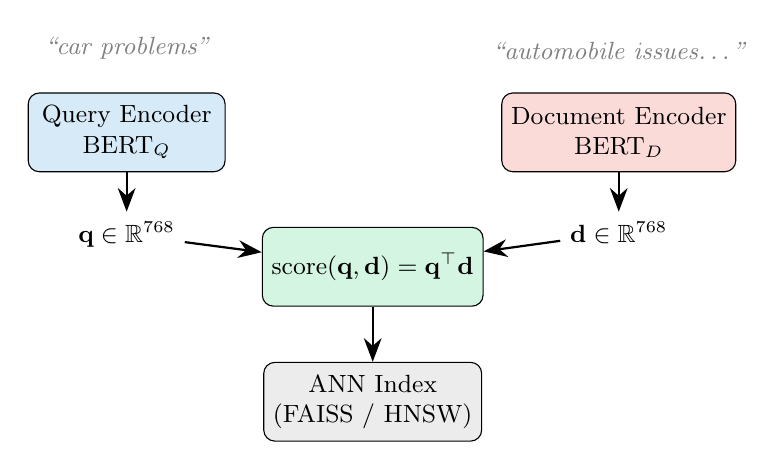
\begin{tikzpicture}[
    box/.style={draw, rounded corners, minimum height=1cm, minimum width=2.5cm, align=center, font=\small},
    arr/.style={-{Stealth[length=3mm]}, thick}
]
\node[box, fill=sparse!20] (qenc) {Query Encoder\\$\text{BERT}_Q$};
\node[box, fill=dense!20, right=3.5cm of qenc] (denc) {Document Encoder\\$\text{BERT}_D$};
\node[below=0.5cm of qenc, font=\small] (q) {$\vq \in \mathbb{R}^{768}$};
\node[below=0.5cm of denc, font=\small] (d) {$\vd \in \mathbb{R}^{768}$};
\node[box, fill=hybrid!20, below=1.2cm of $(qenc)!0.5!(denc)$] (sim) {$\text{score}(\vq,\vd) = \vq^\top \vd$};
\node[box, fill=gray!15, below=0.7cm of sim] (ann) {ANN Index\\(FAISS / HNSW)};

\draw[arr] (qenc) -- (q);
\draw[arr] (denc) -- (d);
\draw[arr] (q) -- (sim);
\draw[arr] (d) -- (sim);
\draw[arr] (sim) -- (ann);

\node[above=0.3cm of qenc, font=\small\itshape, text=gray] {``car problems''};
\node[above=0.3cm of denc, font=\small\itshape, text=gray] {``automobile issues\ldots''};
\end{tikzpicture}
\end{center}

\vspace{0.5em}

\begin{columns}
\begin{column}{0.48\textwidth}
\textbf{Offline (once):}
\begin{itemize}
    \item Encode all 8.8M passages
    \item Build ANN index
    \item $\sim$hours on GPU
\end{itemize}
\end{column}
\begin{column}{0.48\textwidth}
\textbf{Online (per query):}
\begin{itemize}
    \item Encode query: $\sim$5 ms
    \item ANN search: $\sim$10 ms
    \item Total: $\sim$15 ms \textcolor{green}{\checkmark}
\end{itemize}
\end{column}
\end{columns}
\end{frame}

\begin{frame}{Cross-Encoder vs.\ Bi-Encoder}
\begin{center}
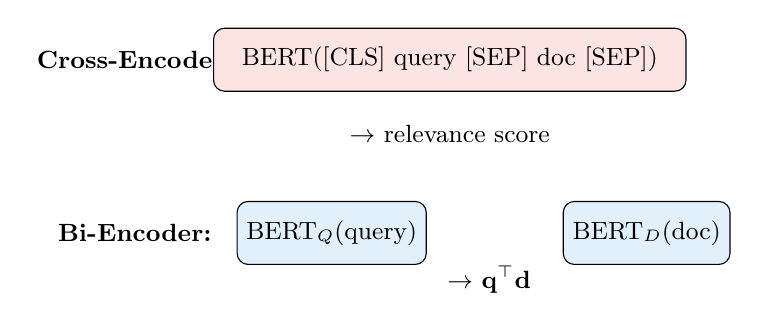
\begin{tikzpicture}[
    box/.style={draw, rounded corners, minimum height=0.8cm, minimum width=2cm, align=center, font=\small},
    arr/.style={-{Stealth[length=2mm]}, thick}
]
% Cross-encoder
\node[font=\small\bfseries] at (-0.5, 2.5) {Cross-Encoder:};
\node[box, fill=dense!15, minimum width=6cm] (ce) at (3.5, 2.5) {BERT([CLS] query [SEP] doc [SEP])};
\node[below=0.3cm of ce, font=\small] {$\to$ relevance score};

% Bi-encoder
\node[font=\small\bfseries] at (-0.5, 0.3) {Bi-Encoder:};
\node[box, fill=sparse!15] (bq) at (2, 0.3) {$\text{BERT}_Q$(query)};
\node[box, fill=sparse!15] (bd) at (6, 0.3) {$\text{BERT}_D$(doc)};
\node[below=0.3cm of $(bq)!0.5!(bd)$, font=\small] {$\to$ $\vq^\top \vd$};
\end{tikzpicture}
\end{center}

\vspace{0.5em}

\begin{table}
\centering
\footnotesize
\begin{tabular}{lcc}
\toprule
& \textbf{Cross-Encoder} & \textbf{Bi-Encoder} \\
\midrule
Query-doc interaction & Full (all layers) & None (dot product only) \\
Pre-compute doc embeddings & \textcolor{red}{\ding{55}} No & \textcolor{green}{\checkmark} Yes (offline) \\
Use for retrieval & \textcolor{red}{\ding{55}} No (too slow) & \textcolor{green}{\checkmark} Yes (with ANN) \\
Accuracy & Higher & Lower \\
Speed at inference & $\sim$5 ms/pair & $\sim$15 ms total \\
\bottomrule
\end{tabular}
\end{table}

\begin{exampleblock}{Key Question}
How do we \textbf{train} the bi-encoder so the dot product captures relevance?
\end{exampleblock}
\end{frame}

% ====================================================================
\section{Contrastive Learning for Retrieval}
% ====================================================================

\begin{frame}[plain]
\sectionpage
\end{frame}

\begin{frame}{Contrastive Learning: Core Principle}
\begin{block}{Objective}
Learn embeddings such that:
$$\text{score}(\vq, \vd^+) \;\gg\; \text{score}(\vq, \vd^-)$$
for relevant pair $(\vq, \vd^+)$ and irrelevant pair $(\vq, \vd^-)$.
\end{block}

\cpause
\vspace{1em}

\textbf{Intuition:} The embedding space is a \textbf{map of meaning}.
\begin{itemize}
    \item ``car problems'' and ``automobile issues'' $\to$ nearby points
    \item ``car problems'' and ``car racing'' $\to$ far apart
\end{itemize}

\cpause
\vspace{0.5em}

\begin{exampleblock}{Connection to Metric Learning}
Define distance $d(\vq, \vd) = 1 - \cos(\vq, \vd)$ and require:
$$d(\vq, \vd^+) + \text{margin} < d(\vq, \vd^-)$$
This is exactly \textbf{deep metric learning} with a learned encoder.
\end{exampleblock}
\end{frame}

\begin{frame}{The InfoNCE Loss}
\begin{block}{InfoNCE / In-Batch Contrastive Loss}
Given query $\vq_i$, positive passage $\vp_i^+$, and $B-1$ in-batch negatives:
$$\mathcal{L} = -\log \frac{\exp\!\bigl(\vq_i^\top \vp_i^+ / \tau\bigr)}{\displaystyle\sum_{j=1}^{B} \exp\!\bigl(\vq_i^\top \vp_j / \tau\bigr)}$$
\end{block}

\cpause
\vspace{0.5em}

\textbf{Key components:}
\begin{itemize}
    \item $B$: batch size --- provides $B-1$ \textbf{free} negatives per query
    \item $\tau$: temperature --- controls sharpness of the softmax
    \item This is $B$-way classification: ``which passage is relevant?''
\end{itemize}

\cpause
\vspace{0.5em}

\begin{alertblock}{No Negative Sampling Needed!}
Unlike traditional LTR, all negatives come for free from the batch. A batch of 128 queries gives 127 negatives per query.
\end{alertblock}
\end{frame}

\begin{frame}{Worked Example: InfoNCE Computation (1/2)}
\textbf{Batch of 3 queries}, each with 1 positive passage ($\tau = 1$):

\vspace{0.5em}

\begin{table}
\centering
\footnotesize
\begin{tabular}{lccc}
\toprule
& $\vp_1$ (``aspirin effects'') & $\vp_2$ (``Tesla founding'') & $\vp_3$ (``Python loops'') \\
\midrule
$\vq_1$ (``aspirin side effects'') & \textbf{0.9} \textcolor{green}{\checkmark} & 0.1 & 0.2 \\
$\vq_2$ (``who founded Tesla'') & 0.15 & \textbf{0.85} \textcolor{green}{\checkmark} & 0.1 \\
$\vq_3$ (``for loops in Python'') & 0.05 & 0.1 & \textbf{0.8} \textcolor{green}{\checkmark} \\
\bottomrule
\end{tabular}
\end{table}

\vspace{0.5em}

\textbf{Similarity matrix} (dot products between query and passage embeddings).

\cpause
\vspace{0.5em}

\textbf{Goal:} Diagonal entries (positives) should dominate each row.
\end{frame}

\begin{frame}{Worked Example: InfoNCE Computation (2/2)}
\textbf{For query $\vq_1$} (``aspirin side effects''):

\vspace{0.5em}

\textbf{Step 1: Exponentiate} ($\tau = 1$):
$$e^{0.9} = 2.46, \quad e^{0.1} = 1.11, \quad e^{0.2} = 1.22$$

\cpause
\vspace{0.5em}

\textbf{Step 2: Softmax} (normalize):
$$P(\vp_1 | \vq_1) = \frac{2.46}{2.46 + 1.11 + 1.22} = \frac{2.46}{4.79} = \mathbf{0.51}$$

\cpause
\vspace{0.5em}

\textbf{Step 3: Loss} (negative log):
$$\mathcal{L}_1 = -\log(0.51) = 0.67$$

\vspace{0.5em}

\begin{exampleblock}{Interpretation}
The model assigns 51\% probability to the correct passage. Training will push this higher by increasing $\vq_1^\top \vp_1$ and decreasing $\vq_1^\top \vp_2$, $\vq_1^\top \vp_3$.
\end{exampleblock}
\end{frame}

\begin{frame}{Temperature Scaling: Why It Matters}
$$p_j = \frac{\exp(s_j / \tau)}{\sum_k \exp(s_k / \tau)}$$

\vspace{0.5em}

\begin{columns}
\begin{column}{0.48\textwidth}
\textbf{Small $\tau$ (e.g., 0.07):}
\begin{itemize}
    \item Distribution becomes \textbf{sharp}
    \item Strong gradients
    \item Risk: training instability
    \item Used by: DPR
\end{itemize}
\end{column}
\begin{column}{0.48\textwidth}
\textbf{Large $\tau$ (e.g., 1.0):}
\begin{itemize}
    \item Distribution becomes \textbf{smooth}
    \item Weaker gradients, more stable
    \item Risk: slow convergence
    \item Used by: ColBERT
\end{itemize}
\end{column}
\end{columns}

\cpause
\vspace{1em}

\begin{alertblock}{Gradient Magnitude}
$\|\nabla \mathcal{L}\| \propto 1/\tau$. Smaller temperature $\to$ stronger signal but training can diverge. This is a critical hyperparameter.
\end{alertblock}
\end{frame}

\begin{frame}{Triplet Loss: The Alternative}
\begin{block}{Triplet Margin Loss}
$$\mathcal{L}_{\text{triplet}} = \max\!\bigl(0,\; d(\vq, \vd^+) - d(\vq, \vd^-) + m\bigr)$$
\end{block}

\vspace{0.5em}

\begin{columns}
\begin{column}{0.48\textwidth}
\textbf{\textcolor{green}{\checkmark} Advantages:}
\begin{itemize}
    \item Explicit margin $m$ enforces separation
    \item Easy to implement
    \item Fast convergence with hard triplets
\end{itemize}
\end{column}
\begin{column}{0.48\textwidth}
\textbf{\textcolor{red}{\ding{55}} Disadvantages:}
\begin{itemize}
    \item Only \textbf{one} negative per anchor
    \item Margin $m$ is a sensitive hyperparameter
    \item Wastes batch information
\end{itemize}
\end{column}
\end{columns}

\cpause
\vspace{1em}

\begin{exampleblock}{In Practice}
InfoNCE dominates because it uses \textbf{all} $B-1$ batch passages as negatives simultaneously --- much richer training signal per step.
\end{exampleblock}
\end{frame}

% ====================================================================
\section{Dense Passage Retrieval (DPR)}
% ====================================================================

\begin{frame}[plain]
\sectionpage
\end{frame}

\begin{frame}{DPR: Architecture (Karpukhin et al., 2020)}
\begin{center}
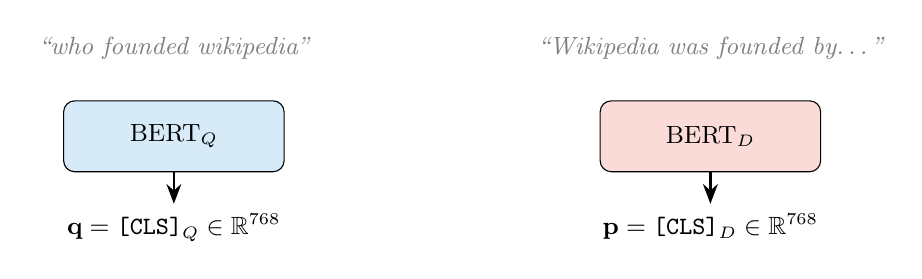
\begin{tikzpicture}[
    box/.style={draw, rounded corners, minimum height=0.9cm, minimum width=2.8cm, align=center, font=\small},
    arr/.style={-{Stealth[length=2.5mm]}, thick}
]
\node[box, fill=sparse!20] (bertq) {$\text{BERT}_Q$};
\node[box, fill=dense!20, right=4cm of bertq] (bertd) {$\text{BERT}_D$};
\node[below=0.4cm of bertq, font=\small] (clsq) {$\vq = \texttt{[CLS]}_Q \in \mathbb{R}^{768}$};
\node[below=0.4cm of bertd, font=\small] (clsd) {$\vp = \texttt{[CLS]}_D \in \mathbb{R}^{768}$};
\node[above=0.4cm of bertq, font=\small\itshape, text=gray] {``who founded wikipedia''};
\node[above=0.4cm of bertd, font=\small\itshape, text=gray] {``Wikipedia was founded by\ldots''};

\draw[arr] (bertq) -- (clsq);
\draw[arr] (bertd) -- (clsd);
\end{tikzpicture}
\end{center}

\vspace{0.5em}

\begin{block}{Key Design Choices}
\begin{itemize}
    \item \textbf{Separate encoders:} $\text{BERT}_Q \neq \text{BERT}_D$ (different weights, can specialize)
    \item \textbf{Representation:} \texttt{[CLS]} token output --- single vector per text
    \item \textbf{Similarity:} $\text{score}(\vq, \vp) = \vq^\top \vp$ (dot product)
    \item \textbf{No interaction:} Query and passage never ``see'' each other during encoding
\end{itemize}
\end{block}
\end{frame}

\begin{frame}{DPR: Training Recipe}
\begin{columns}[T]
\begin{column}{0.55\textwidth}
\textbf{Loss:} InfoNCE with in-batch negatives
$$\mathcal{L} = -\log \frac{e^{\vq_i^\top \vp_i^+/\tau}}{\sum_{j=1}^{B} e^{\vq_i^\top \vp_j / \tau}}$$

\vspace{0.5em}

\textbf{Negatives per query:}
\begin{enumerate}
    \item $B-1$ in-batch negatives (free!)
    \item 1 BM25 hard negative (precomputed)
\end{enumerate}
\end{column}

\begin{column}{0.42\textwidth}
\begin{table}
\footnotesize
\begin{tabular}{ll}
\toprule
\textbf{Param} & \textbf{Value} \\
\midrule
Batch size & 128 \\
Temperature $\tau$ & 1.0 \\
Learning rate & $10^{-5}$ \\
Epochs & 40 \\
Optimizer & Adam \\
Max $|q|$ & 64 tokens \\
Max $|p|$ & 256 tokens \\
\bottomrule
\end{tabular}
\end{table}
\end{column}
\end{columns}

\cpause
\vspace{0.5em}

\begin{exampleblock}{Key Insight}
Mixing \textbf{one} BM25 hard negative with in-batch random negatives is surprisingly effective. The BM25 negative is lexically similar but not relevant --- forces the model beyond surface matching.
\end{exampleblock}
\end{frame}

\begin{frame}{DPR: Why BM25 Hard Negatives?}
\textbf{Query:} ``side effects of aspirin''

\vspace{1em}

\textbf{Random negative:} ``The capital of France is Paris\ldots''
\begin{itemize}
    \item $\vq^\top \vd^- \approx 0.05$ --- trivially easy, \textbf{no learning signal}
\end{itemize}

\cpause
\vspace{0.5em}

\textbf{BM25 hard negative:} ``Aspirin was invented by Bayer in 1899\ldots''
\begin{itemize}
    \item Contains ``aspirin'' $\to$ BM25 ranks it high
    \item But \textbf{not about side effects} $\to$ not relevant
    \item $\vq^\top \vd^- \approx 0.6$ --- confusing, \textbf{strong learning signal!}
\end{itemize}

\cpause
\vspace{1em}

\begin{alertblock}{The Principle}
The model must learn: ``just because a passage mentions aspirin doesn't mean it's about side effects.'' This is \textbf{exactly} what BM25 cannot do.
\end{alertblock}
\end{frame}

\begin{frame}{DPR: Results \& Significance}
\begin{center}
\begin{tabular}{lccc}
\toprule
\textbf{Method} & \textbf{NQ Top-20 Recall} & \textbf{MS MARCO MRR@10} & \textbf{Params} \\
\midrule
BM25 & 59.1 & 18.7 & --- \\
\textbf{DPR} & \textbf{78.4} & \textbf{31.1} & 220M \\
\bottomrule
\end{tabular}
\end{center}

\vspace{1em}

\begin{block}{Why DPR Matters}
\begin{itemize}
    \item First system to conclusively show \textbf{dense $>$ sparse} for open-domain QA
    \item +19pp top-20 recall over BM25 on Natural Questions
    \item Enabled the modern ``retriever + reader'' paradigm
\end{itemize}
\end{block}

\cpause
\vspace{0.5em}

\begin{alertblock}{But\ldots}
A single 768-dim vector for the entire document? That's a severe \textbf{information bottleneck}. Can we do better?
\end{alertblock}
\end{frame}

% ====================================================================
\section{ColBERT: Late Interaction}
% ====================================================================

\begin{frame}[plain]
\sectionpage
\end{frame}

\begin{frame}{The Single-Vector Bottleneck}
\begin{alertblock}{Problem with DPR}
The \textbf{entire} document is compressed into a single 768-dim vector.
\end{alertblock}

\vspace{0.5em}

\begin{center}
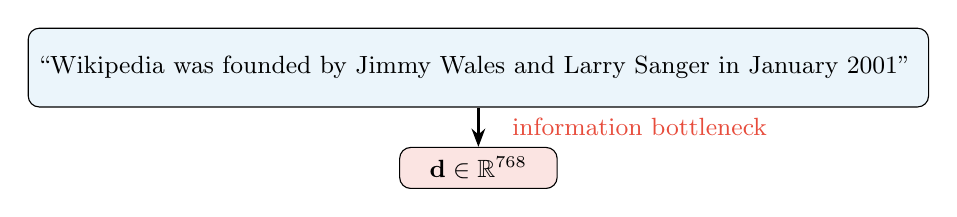
\begin{tikzpicture}[font=\small]
\node[draw, fill=sparse!10, rounded corners, minimum width=9cm, minimum height=1cm, align=center] (doc) {
    ``Wikipedia was founded by Jimmy Wales and Larry Sanger in January 2001''
};
\node[draw, fill=dense!15, rounded corners, minimum width=2cm, below=0.5cm of doc] (vec) {$\vd \in \mathbb{R}^{768}$};
\draw[-{Stealth}, thick] (doc) -- (vec) node[midway, right, xshift=0.3cm] {\textcolor{dense}{information bottleneck}};
\end{tikzpicture}
\end{center}

\cpause
\vspace{0.5em}

\textbf{Consequences:}
\begin{itemize}
    \item Cannot capture fine-grained token-level alignments
    \item ``\textbf{Who} founded Wikipedia?'' vs.\ ``\textbf{When} was Wikipedia founded?'' $\to$ similar scores!
    \item Long documents lose information
\end{itemize}

\cpause
\vspace{0.5em}

\begin{exampleblock}{Solution}
Keep \textbf{all} token embeddings, not just \texttt{[CLS]}. Compare at the token level.
\end{exampleblock}
\end{frame}

\begin{frame}[fragile]{ColBERT: Architecture (Khattab \& Zaharia, 2020)}
\begin{block}{Key Idea}
Encode query and document \textbf{separately} (like bi-encoder), but compare at the \textbf{token level} using MaxSim.
\end{block}

\vspace{0.5em}

\begin{center}
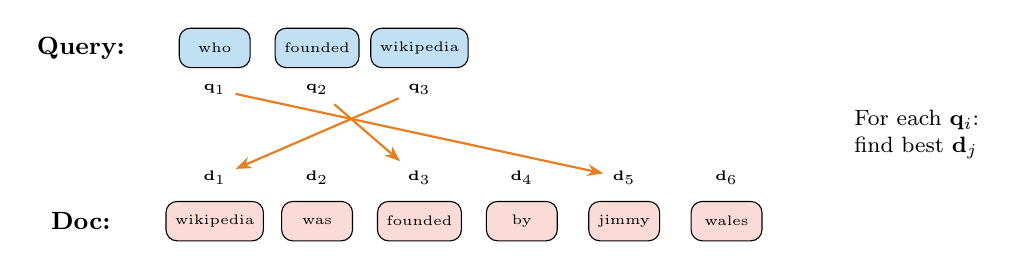
\begin{tikzpicture}[
    tok/.style={draw, rounded corners, fill=#1, minimum width=0.9cm, minimum height=0.5cm, font=\tiny},
    arr/.style={-{Stealth[length=2mm]}, thin, gray}
]
% Query tokens
\node[font=\small\bfseries] at (-1.2, 2.2) {Query:};
\foreach \i/\w/\c in {0/who/sparse!30, 1/founded/sparse!30, 2/wikipedia/sparse!30} {
    \node[tok=\c] (q\i) at (1.3*\i + 0.5, 2.2) {\w};
    \node[font=\tiny, below=0.08cm of q\i] (qe\i) {$\vq_{\the\numexpr\i+1}$};
}

% Doc tokens
\node[font=\small\bfseries] at (-1.2, 0) {Doc:};
\foreach \i/\w/\c in {0/wikipedia/dense!20, 1/was/dense!20, 2/founded/dense!20, 3/by/dense!20, 4/jimmy/dense!20, 5/wales/dense!20} {
    \node[tok=\c] (d\i) at (1.3*\i + 0.5, 0) {\w};
    \node[font=\tiny, above=0.08cm of d\i] (de\i) {$\vd_{\the\numexpr\i+1}$};
}

% MaxSim arrows (best matches)
\draw[arr, thick, dense] (qe0) -- (de4);
\draw[arr, thick, dense] (qe1) -- (de2);
\draw[arr, thick, dense] (qe2) -- (de0);

\node[font=\footnotesize, anchor=west, align=left] at (8.5, 1.1) {For each $\vq_i$:\\find best $\vd_j$};
\end{tikzpicture}
\end{center}

\cpause
\vspace{0.3em}

\begin{exampleblock}{Late Interaction}
Documents are encoded \textbf{offline} (token-level embeddings stored). The ``interaction'' happens \textbf{late} --- only at query time via MaxSim.
\end{exampleblock}
\end{frame}

\begin{frame}{ColBERT: MaxSim Scoring}
\begin{block}{MaxSim Definition}
$$\text{MaxSim}(\vq, \vd) = \sum_{i=1}^{|\vq|} \max_{j=1}^{|\vd|}\; \cos(\vq_i, \vd_j)$$
\end{block}

\vspace{0.5em}

\textbf{Step by step:}
\begin{enumerate}
    \item For each query token $\vq_i$, find the document token $\vd_j$ with highest cosine similarity
    \item Take that maximum similarity
    \item Sum across all query tokens
\end{enumerate}

\cpause
\vspace{0.5em}

\textbf{Properties:}
\begin{itemize}
    \item \textbf{Asymmetric:} Every query token must find a match; document tokens can be ignored
    \item \textbf{Decomposable:} Document embeddings precomputed and stored offline
    \item Token embeddings: $\vq_i, \vd_j \in \mathbb{R}^{128}$ (projected down from 768)
\end{itemize}
\end{frame}

\begin{frame}{Worked Example: MaxSim Scoring}
\textbf{Query:} ``who founded wikipedia'' (3 tokens)\\
\textbf{Document:} ``wikipedia was founded by jimmy wales'' (6 tokens)

\vspace{0.5em}

\begin{table}
\centering
\footnotesize
\begin{tabular}{lcccccc}
\toprule
& \textit{wikipedia} & \textit{was} & \textit{founded} & \textit{by} & \textit{jimmy} & \textit{wales} \\
\midrule
\textit{who}       & 0.12 & 0.08 & 0.15 & 0.10 & \textbf{0.72} & 0.45 \\
\textit{founded}   & 0.20 & 0.05 & \textbf{0.95} & 0.10 & 0.12 & 0.08 \\
\textit{wikipedia} & \textbf{0.98} & 0.06 & 0.18 & 0.04 & 0.10 & 0.15 \\
\bottomrule
\end{tabular}
\end{table}

\cpause
\vspace{0.5em}

$$\text{MaxSim} = \underbrace{0.72}_{\text{who}\to\text{jimmy}} + \underbrace{0.95}_{\text{founded}\to\text{founded}} + \underbrace{0.98}_{\text{wikipedia}\to\text{wikipedia}} = \mathbf{2.65}$$

\vspace{0.5em}

\begin{exampleblock}{Notice}
``who'' aligns with ``jimmy'' (the answer entity) --- the model learns \textbf{semantic alignment}, not just exact matching.
\end{exampleblock}
\end{frame}

\begin{frame}{ColBERT: Efficiency vs.\ Accuracy}
\begin{table}
\centering
\small
\begin{tabular}{lccc}
\toprule
& \textbf{DPR (Bi-Enc)} & \textbf{ColBERT} & \textbf{Cross-Encoder} \\
\midrule
Interaction & None (dot prod) & Late (MaxSim) & Full (cross-attn) \\
Pre-compute docs & \textcolor{green}{\checkmark} (1 vec) & \textcolor{green}{\checkmark} ($n$ vecs) & \textcolor{red}{\ding{55}} \\
Use for retrieval & \textcolor{green}{\checkmark} With ANN & \textcolor{green}{\checkmark} With ANN & \textcolor{red}{\ding{55}} Too slow \\
Speedup vs.\ CE & $\sim$1000$\times$ & $\sim$100$\times$ & $1\times$ \\
MS MARCO MRR@10 & 31.1 & 36.0 & 39.0 \\
Storage per doc & $768 \times 4$B = 3 KB & $128 \times 128 \times 4$B $\approx$ 64 KB & N/A \\
\bottomrule
\end{tabular}
\end{table}

\cpause
\vspace{0.5em}

\begin{exampleblock}{Sweet Spot}
ColBERT gives near-cross-encoder accuracy at bi-encoder-like speed. Trade-off: \textbf{much higher storage} (one vector per token, not per document).
\end{exampleblock}
\end{frame}

% ====================================================================
\section{ANCE: Dynamic Hard Negatives}
% ====================================================================

\begin{frame}[plain]
\sectionpage
\end{frame}

\begin{frame}{The Hard Negative Problem (Xiong et al., 2021)}
\begin{alertblock}{Observation}
Most in-batch negatives are \textbf{trivially easy}. The model separates them instantly and stops learning.
\end{alertblock}

\vspace{0.5em}

\begin{center}
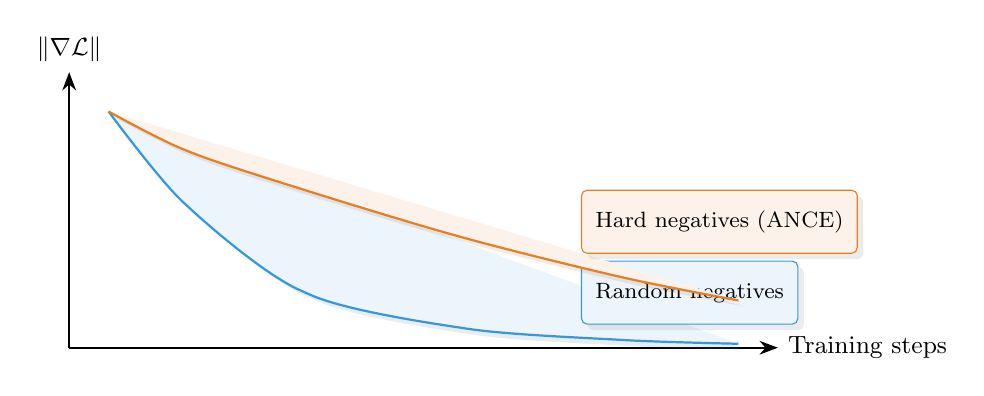
\begin{tikzpicture}[font=\small]
\draw[-{Stealth}, thick] (0,0) -- (9,0) node[right] {Training steps};
\draw[-{Stealth}, thick] (0,0) -- (0,3.5) node[above] {$\|\nabla \mathcal{L}\|$};

\draw[sparse, thick] plot[smooth] coordinates {(0.5,3) (1.5,1.8) (3,0.7) (5,0.25) (7,0.1) (8.5,0.05)};
\node[sparse, font=\footnotesize, anchor=west] at (6.5,0.7) {Random negatives};

\draw[dense, thick] plot[smooth] coordinates {(0.5,3) (1.5,2.5) (3,2) (5,1.4) (7,0.9) (8.5,0.6)};
\node[dense, font=\footnotesize, anchor=west] at (6.5,1.6) {Hard negatives (ANCE)};
\end{tikzpicture}
\end{center}

\cpause
\vspace{0.3em}

Random negatives $\Rightarrow$ gradients vanish early $\Rightarrow$ \textbf{slow convergence, wasted compute}.
\end{frame}

\begin{frame}[fragile]{ANCE: Asynchronous Index Refresh}
\begin{block}{Core Innovation}
Maintain an ANN index during training. Use the model's \textbf{own} top-$k$ nearest passages as hard negatives.
\end{block}

\vspace{0.5em}

\begin{center}
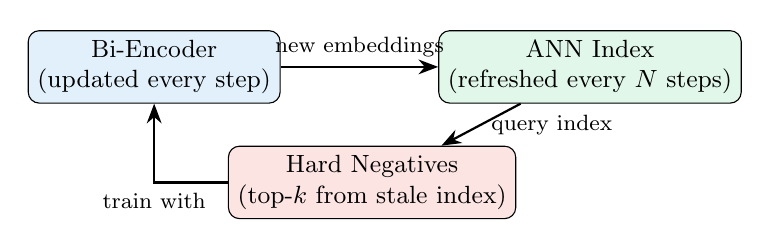
\begin{tikzpicture}[
    box/.style={draw, rounded corners, fill=#1, minimum height=0.8cm, minimum width=2.8cm, align=center, font=\small},
    arr/.style={-{Stealth[length=2.5mm]}, thick}
]
\node[box=sparse!15] (enc) {Bi-Encoder\\(updated every step)};
\node[box=hybrid!15, right=2cm of enc] (idx) {ANN Index\\(refreshed every $N$ steps)};
\node[box=dense!15, below=1cm of $(enc)!0.5!(idx)$] (neg) {Hard Negatives\\(top-$k$ from stale index)};

\draw[arr] (enc) -- (idx) node[midway, above, font=\footnotesize] {new embeddings};
\draw[arr] (idx) -- (neg) node[midway, right, font=\footnotesize] {query index};
\draw[arr] (neg) -| (enc) node[midway, below, font=\footnotesize] {train with};
\end{tikzpicture}
\end{center}

\cpause
\vspace{0.3em}

\begin{exampleblock}{Why the Lag is a Feature}
The index lags by $N$ steps. Negatives are hard (from a recent model) but not \textbf{impossibly} hard (from the current model). This stabilizes training.
\end{exampleblock}
\end{frame}

\begin{frame}{ANCE: Gradient Analysis}
\begin{block}{Why Hard Negatives Produce Better Gradients}
The gradient of InfoNCE w.r.t.\ $\vq$ decomposes as:
$$\frac{\partial \mathcal{L}}{\partial \vq} = \underbrace{(p^+ - 1) \cdot \vp^+}_{\text{pull toward positive}} + \underbrace{\sum_{j \neq +} p_j \cdot \vp_j}_{\text{push from negatives}}$$
where $p_j = \text{softmax}(\vq^\top \vp_j / \tau)$.
\end{block}

\cpause
\vspace{0.5em}

\begin{columns}
\begin{column}{0.48\textwidth}
\textbf{Easy negatives:}
\begin{itemize}
    \item $p_j \approx 0$ for all $j \neq +$
    \item Push terms \textbf{vanish}
    \item No learning signal
\end{itemize}
\end{column}
\begin{column}{0.48\textwidth}
\textbf{Hard negatives:}
\begin{itemize}
    \item $p_j > 0$ for confusing $j$
    \item Push terms are \textbf{large}
    \item Strong, informative gradient
\end{itemize}
\end{column}
\end{columns}
\end{frame}

\begin{frame}{ANCE: Results}
\begin{center}
\begin{tabular}{lccc}
\toprule
\textbf{Method} & \textbf{NQ Top-20 R} & \textbf{MS MARCO MRR@10} & \textbf{Negatives} \\
\midrule
BM25 & 59.1 & 18.7 & --- \\
DPR (BM25 neg.) & 78.4 & 31.1 & Static / lexical \\
\textbf{ANCE} & \textbf{81.9} & \textbf{33.0} & Dynamic / semantic \\
\bottomrule
\end{tabular}
\end{center}

\cpause
\vspace{1em}

\begin{exampleblock}{Key Takeaway}
The \textbf{only} difference between DPR and ANCE is the negative sampling strategy. Semantic hard negatives from the model's own index are strictly better than BM25 hard negatives.
\end{exampleblock}

\begin{alertblock}{Implication}
Negative sampling is a \textbf{first-order concern} in dense retrieval. The model, the loss, and the architecture are the same --- it's the negatives that matter most.
\end{alertblock}
\end{frame}

% ====================================================================
\section{Training Dense Retrievers in Practice}
% ====================================================================

\begin{frame}[plain]
\sectionpage
\end{frame}

\begin{frame}{Negative Sampling Strategies}
\begin{block}{The Core Question}
Query has 1 labeled positive. Where do the negatives come from?
\end{block}

\vspace{0.5em}

\begin{enumerate}
    \item \textbf{Random negatives}
    \begin{itemize}
        \item Sample random passage from corpus
        \item Easy to distinguish $\to$ weak training signal
        \item \textcolor{red}{\ding{55}} Not recommended for production
    \end{itemize}

    \cpause
    \vspace{0.3em}

    \item \textbf{BM25 hard negatives} \textcolor{green}{\checkmark} \textit{Good starting point}
    \begin{itemize}
        \item Top-$k$ BM25 results that are \textit{not} labeled relevant
        \item Lexically similar but semantically different $\to$ strong signal
    \end{itemize}

    \cpause
    \vspace{0.3em}

    \item \textbf{ANN hard negatives (ANCE)} \textcolor{green}{\checkmark} \textit{Best quality}
    \begin{itemize}
        \item Top-$k$ from model's own index (refreshed periodically)
        \item Semantically hard --- forces fine-grained distinctions
    \end{itemize}
\end{enumerate}
\end{frame}

\begin{frame}{The False Negative Problem}
\begin{alertblock}{Issue}
In-batch negatives may actually be \textbf{relevant} (but unlabeled).
\end{alertblock}

\vspace{0.5em}

\textbf{Example:} Query ``Who founded Wikipedia?''
\begin{itemize}
    \item \textbf{Labeled positive:} ``Wikipedia was founded by Jimmy Wales and Larry Sanger\ldots''
    \item \textbf{In-batch ``negative'':} ``Jimmy Wales co-founded Wikipedia in 2001\ldots''\\
    $\leftarrow$ \textcolor{dense}{Actually relevant! But treated as negative.}
\end{itemize}

\cpause
\vspace{0.5em}

\textbf{Consequence:} Model penalized for correctly ranking a relevant passage high.

\vspace{0.5em}

\begin{exampleblock}{Mitigations}
\begin{itemize}
    \item Confidence regularization: down-weight uncertain negatives
    \item Larger corpora reduce false negative probability
    \item Cross-encoder denoising (re-score negatives, remove false ones)
\end{itemize}
\end{exampleblock}
\end{frame}

\begin{frame}{Training Hyperparameters}
\begin{columns}
\begin{column}{0.48\textwidth}
\textbf{Batching \& Memory}
\begin{itemize}
    \item Max sequence: 256 tokens (passage)
    \item Batch size: 128 (critical!)
    \item \textbf{Larger batch = more negatives = better}
    \item Gradient accumulation to simulate larger batches
    \item Mixed precision (fp16) saves $\sim$50\% memory
\end{itemize}
\end{column}

\begin{column}{0.48\textwidth}
\textbf{Optimization}
\begin{itemize}
    \item Learning rate: $1$--$3 \times 10^{-5}$
    \item Warmup: 10\% of steps
    \item Scheduler: linear decay
    \item Epochs: 20--40
    \item Temperature $\tau$: 0.05--1.0
    \item Evaluate every 5K steps
\end{itemize}
\end{column}
\end{columns}

\cpause
\vspace{1em}

\begin{alertblock}{Key Difference from Cross-Encoder Training}
Batch size matters \textbf{much more} for bi-encoders. Each additional batch element provides a free negative. Going from batch 32 to 128 can improve MRR by 2--3 points.
\end{alertblock}
\end{frame}

\begin{frame}{Common Training Mistakes}
\begin{alertblock}{Avoid These Pitfalls}
\begin{enumerate}
    \item \textbf{Batch size too small}
    \begin{itemize}
        \item Batch 16 = only 15 negatives per query
        \item Use gradient accumulation to simulate larger batches
    \end{itemize}

    \item \textbf{Only random negatives}
    \begin{itemize}
        \item Model never sees hard cases $\to$ weak representations
        \item Always include BM25 or ANN hard negatives
    \end{itemize}

    \item \textbf{Wrong temperature}
    \begin{itemize}
        \item Too small: training diverges
        \item Too large: convergence too slow
        \item Start with $\tau = 0.05$, tune on dev set
    \end{itemize}

    \item \textbf{Not normalizing embeddings}
    \begin{itemize}
        \item Without L2 normalization, embedding magnitudes grow unbounded
        \item Always normalize before computing similarity
    \end{itemize}
\end{enumerate}
\end{alertblock}
\end{frame}

\begin{frame}[fragile]{Training Code Sketch (Hugging Face + Sentence-Transformers)}
\begin{lstlisting}[language=Python]
from sentence_transformers import SentenceTransformer
from sentence_transformers import InputExample, losses

# Load pre-trained bi-encoder
model = SentenceTransformer('bert-base-uncased')

# Create training pairs
train_examples = [
    InputExample(texts=[query, pos_passage, neg_passage])
    for query, pos_passage, neg_passage in triples
]

# MultipleNegativesRankingLoss = InfoNCE
train_loss = losses.MultipleNegativesRankingLoss(model)

# Train
model.fit(
    train_objectives=[(train_dataloader, train_loss)],
    epochs=10,
    warmup_steps=1000,
    evaluation_steps=5000,
)
\end{lstlisting}
\end{frame}

% ====================================================================
\section{Theoretical Foundations}
% ====================================================================

\begin{frame}[plain]
\sectionpage
\end{frame}

\begin{frame}{Why Does Contrastive Learning Work?}
\begin{block}{InfoNCE as Mutual Information Lower Bound (Oord et al., 2018)}
$$I(\vq; \vd^+) \;\geq\; \log(B) - \mathcal{L}_{\text{InfoNCE}}$$
\end{block}

\vspace{0.5em}

\textbf{Interpretation:} Minimizing InfoNCE \textbf{maximizes} a lower bound on mutual information between query and positive document embeddings.

\cpause
\vspace{0.5em}

\begin{exampleblock}{Why This Matters for Retrieval}
\begin{itemize}
    \item High $I(\vq; \vd^+)$: query embedding is \textbf{predictive} of relevant documents
    \item The bound is tighter with more negatives (larger $B$)
    \item This explains why \textbf{large batch sizes help}: tighter MI bound
\end{itemize}
\end{exampleblock}
\end{frame}

\begin{frame}[fragile]{The Information Bottleneck Perspective}
\begin{block}{IB Objective (Tishby et al., 2000)}
$$\min_T \;\bigl[\beta \cdot I(T; X) - I(T; Y)\bigr]$$
\end{block}

\vspace{0.5em}

\begin{center}
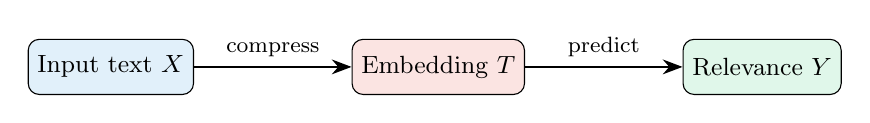
\begin{tikzpicture}[
    box/.style={draw, rounded corners, fill=#1, minimum width=2cm, minimum height=0.7cm, align=center, font=\small},
    arr/.style={-{Stealth[length=2.5mm]}, thick}
]
\node[box=sparse!15] (x) {Input text $X$};
\node[box=dense!15, right=2cm of x] (t) {Embedding $T$};
\node[box=hybrid!15, right=2cm of t] (y) {Relevance $Y$};

\draw[arr] (x) -- (t) node[midway, above, font=\footnotesize] {compress};
\draw[arr] (t) -- (y) node[midway, above, font=\footnotesize] {predict};
\end{tikzpicture}
\end{center}

\cpause
\vspace{0.5em}

\begin{itemize}
    \item $I(T; Y)$ \textbf{high}: Embedding retains what's needed for relevance
    \item $I(T; X)$ \textbf{low}: Embedding discards noise and irrelevant features
\end{itemize}

\vspace{0.5em}

\begin{exampleblock}{Implication}
Dense retrieval generalizes because the bottleneck forces the model to learn \textbf{essential semantic features}, not surface patterns.
\end{exampleblock}
\end{frame}

\begin{frame}{Representation Collapse}
\begin{alertblock}{Definition}
All embeddings converge to a single point (or low-rank subspace):
$$\forall\, i,j: \;\; \|\vd_i - \vd_j\| \to 0 \quad\Rightarrow\quad \text{score}(\vq, \vd_i) \approx \text{score}(\vq, \vd_j)$$
\end{alertblock}

\cpause
\vspace{0.5em}

\textbf{Two collapse modes:}
\begin{enumerate}
    \item \textbf{Complete collapse:} All embeddings map to $\mathbf{0}$\\
    {\small Cause: no negatives $\Rightarrow$ trivial zero-loss solution}

    \item \textbf{Dimensional collapse:} Embeddings use only a few dimensions\\
    {\small Cause: easy negatives $\Rightarrow$ only coarse features needed}
\end{enumerate}

\cpause
\vspace{0.5em}

\begin{exampleblock}{Prevention}
\textbf{Hard negatives} + $\ell_2$ normalization + proper temperature. Hard negatives force the model to use all dimensions $\to$ prevents collapse.
\end{exampleblock}
\end{frame}

\begin{frame}{Neural Collapse \& Optimal Geometry (Papyan et al., 2020)}
\begin{block}{Equiangular Tight Frame (ETF)}
In the terminal phase of training, class means $\{\boldsymbol{\mu}_c\}$ form a maximally symmetric structure:
$$\boldsymbol{\mu}_i^\top \boldsymbol{\mu}_j = \begin{cases}
1 & i = j \\
-\frac{1}{C-1} & i \neq j
\end{cases}$$
\end{block}

\vspace{0.5em}

\textbf{Properties:}
\begin{itemize}
    \item All class centers are \textbf{equidistant} (maximally separated)
    \item Points collapse to their class mean (minimal within-class variance)
    \item \textbf{Maximum margin} between all classes
\end{itemize}

\cpause
\vspace{0.5em}

\begin{exampleblock}{Relevance to Retrieval}
Hard negatives push representations toward ETF geometry. Without them, dimensional collapse prevents this optimal structure from forming.
\end{exampleblock}
\end{frame}

% ====================================================================
\section{Evaluation \& The Zero-Shot Challenge}
% ====================================================================

\begin{frame}[plain]
\sectionpage
\end{frame}

\begin{frame}{Key Benchmarks}
\begin{table}
\centering
\small
\begin{tabular}{lccl}
\toprule
\textbf{Benchmark} & \textbf{Corpus} & \textbf{Queries} & \textbf{Primary Metric} \\
\midrule
MS MARCO & 8.8M passages & 500K train & MRR@10 \\
Natural Questions & 21M passages & 3.5K test & Top-20 Recall \\
BEIR (18 tasks) & Varies & Varies & nDCG@10 (zero-shot) \\
TREC-DL 2019/20 & 8.8M passages & 43/54 & nDCG@10 \\
\bottomrule
\end{tabular}
\end{table}

\cpause
\vspace{0.5em}

\begin{alertblock}{Critical Distinction}
\begin{itemize}
    \item MS MARCO / NQ: \textbf{In-domain} (train \& test same distribution)
    \item BEIR: \textbf{Zero-shot} (train on MS MARCO, test on 18 diverse tasks)
    \item Dense methods excel in-domain but often struggle on BEIR!
\end{itemize}
\end{alertblock}
\end{frame}

\begin{frame}{The Zero-Shot Challenge: BEIR}
\begin{center}
\begin{tabular}{lccccc}
\toprule
& \textbf{BM25} & \textbf{DPR} & \textbf{ColBERT} & \textbf{ANCE} & \textbf{Contriever} \\
\midrule
BEIR Avg nDCG@10 & 47.3 & 33.2 & 41.5 & 37.7 & 48.5 \\
\bottomrule
\end{tabular}
\end{center}

\cpause
\vspace{0.5em}

\begin{alertblock}{Surprising Finding}
\textbf{BM25 outperforms} most dense models on zero-shot BEIR!
\end{alertblock}

\textbf{Why?}
\begin{itemize}
    \item Dense models overfit to NQ/MS MARCO query structure
    \item BM25 is distribution-agnostic (just uses term statistics)
    \item BEIR includes fact-checking, citation prediction, argument retrieval
\end{itemize}

\cpause
\vspace{0.5em}

\begin{exampleblock}{Solution: Contriever (Izacard et al., 2022)}
Unsupervised contrastive pre-training on diverse data \textbf{before} fine-tuning. Achieves 48.5 --- finally beating BM25 on BEIR.
\end{exampleblock}
\end{frame}

\begin{frame}{Hybrid Retrieval: Dense + Sparse}
\begin{block}{Key Finding}
Combining BM25 and dense retrieval \textbf{outperforms either alone}.
\end{block}

\vspace{0.5em}

$$\text{score}_{\text{hybrid}}(q, d) = \alpha \cdot \text{score}_{\text{BM25}}(q,d) + (1-\alpha) \cdot \text{score}_{\text{dense}}(q,d)$$

\vspace{0.5em}

\begin{center}
\begin{tabular}{lc}
\toprule
\textbf{Method} & \textbf{NQ Top-20 Recall} \\
\midrule
BM25 alone & 62.9 \\
DPR alone & 78.4 \\
BM25 + DPR (hybrid) & \textbf{82.6} \\
\bottomrule
\end{tabular}
\end{center}

\cpause
\vspace{0.5em}

\begin{exampleblock}{Why Hybrid Works}
Sparse captures \textbf{exact matches} (named entities, rare terms). Dense captures \textbf{semantic similarity} (paraphrases). They are complementary, not competing.
\end{exampleblock}
\end{frame}

% ====================================================================
\section{Hands-On with PyTerrier}
% ====================================================================

\begin{frame}[plain]
\sectionpage
\end{frame}

\begin{frame}[fragile]{Setup: Dense Retrieval with PyTerrier}
\begin{lstlisting}[language=Python]
import pyterrier as pt
if not pt.started():
    pt.init()

dataset = pt.get_dataset('irds:msmarco-passage/dev/small')
topics = dataset.get_topics().head(50)
qrels = dataset.get_qrels()

# BM25 baseline
index = pt.IndexFactory.of("./msmarco_index")
bm25 = pt.BatchRetrieve(index, wmodel="BM25")

# Dense retrieval with ANCE
from pyterrier_dr import FlexIndex, TctColBert

# Load pre-trained dense encoder
encoder = TctColBert()  # or ANCE, DPR, etc.
flex_index = FlexIndex("./dense_index")

# Dense retriever
dense = encoder >> flex_index
\end{lstlisting}
\end{frame}

\begin{frame}[fragile]{Exercise 1: BM25 vs.\ Dense Retrieval}
\begin{lstlisting}[language=Python]
# Compare BM25 vs. Dense vs. Hybrid
hybrid = (bm25 % 1000) | (dense % 1000)  # union

comparison = pt.Experiment(
    [bm25, dense, hybrid],
    topics, qrels,
    eval_metrics=["map", "ndcg_cut_10", "recall_100"],
    names=["BM25", "Dense (ANCE)", "Hybrid"]
)
print(comparison)
\end{lstlisting}

\vspace{0.5em}

\textbf{Questions to explore:}
\begin{itemize}
    \item Which queries does dense retrieval improve on?
    \item Which queries does BM25 still win?
    \item How much does hybrid add over each individual method?
\end{itemize}
\end{frame}

\begin{frame}[fragile]{Exercise 2: Dense + Cross-Encoder Pipeline}
\begin{lstlisting}[language=Python]
from pyterrier_t5 import MonoT5ReRanker

monoT5 = MonoT5ReRanker(model='castorini/monot5-base-msmarco')

# Three-stage pipeline: Dense -> Cross-Encoder
pipeline_dense_ce = (dense % 100) >> monoT5

# Compare all variants
results = pt.Experiment(
    [bm25,
     (bm25 % 100) >> monoT5,       # L4 pipeline
     dense,
     pipeline_dense_ce,              # New: dense + CE
     (hybrid % 100) >> monoT5],     # Best of all worlds
    topics, qrels,
    eval_metrics=["ndcg_cut_10", "recall_100"],
    names=["BM25", "BM25+monoT5", "Dense",
           "Dense+monoT5", "Hybrid+monoT5"]
)
\end{lstlisting}
\end{frame}

\begin{frame}{Student Exercises}
\begin{block}{Exercise A: Semantic vs.\ Lexical Analysis (10 min)}
\begin{itemize}
    \item Find a query where dense retrieval finds relevant docs that BM25 missed
    \item Inspect: is it vocabulary mismatch? Paraphrase? Different phrasing?
    \item Compare the top-5 results from each
\end{itemize}
\end{block}

\begin{block}{Exercise B: When Dense Fails (10 min)}
\begin{itemize}
    \item Find a query where BM25 beats dense retrieval
    \item Check: is it an entity name? Rare technical term? Exact match needed?
    \item Would hybrid retrieval fix it?
\end{itemize}
\end{block}

\begin{block}{Exercise C: Recall Ceiling (5 min)}
\begin{itemize}
    \item Compare Recall@1000 of BM25 vs.\ dense vs.\ hybrid
    \item Which gives the best ceiling for the cross-encoder re-ranker?
    \item Connect back to Lecture 4: the recall ceiling determines the pipeline's upper bound
\end{itemize}
\end{block}
\end{frame}

% ====================================================================
\section{Connections and Summary}
% ====================================================================

\begin{frame}[plain]
\sectionpage
\end{frame}

\begin{frame}[fragile]{The Complete Modern Retrieval Stack}
\begin{center}
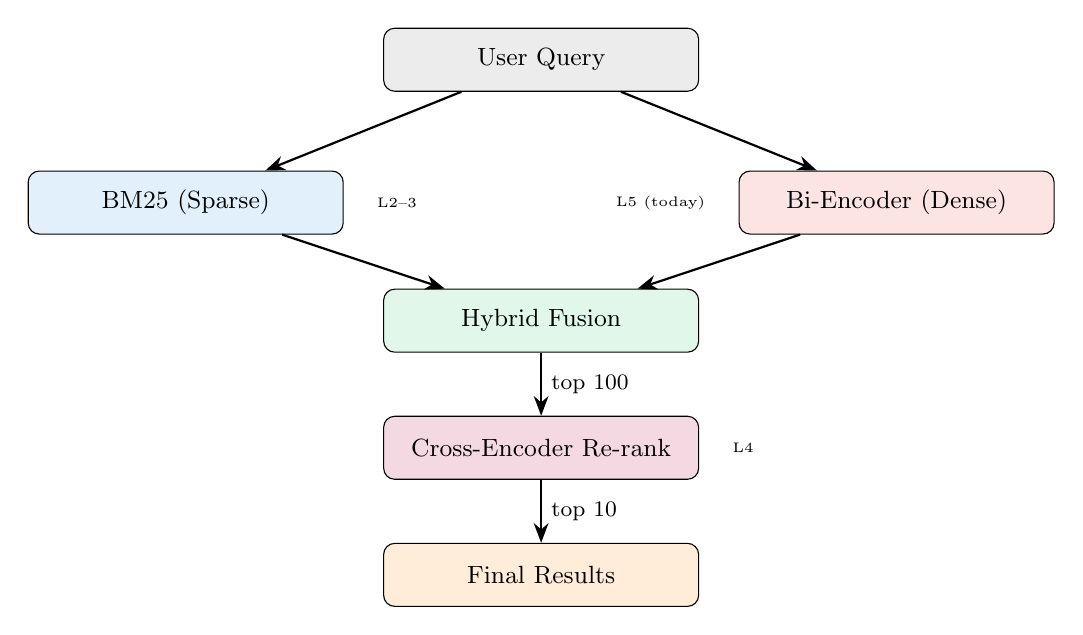
\begin{tikzpicture}[
    box/.style={draw, rounded corners, fill=#1, minimum height=0.8cm, minimum width=4cm, align=center, font=\small},
    arr/.style={-{Stealth[length=2.5mm]}, thick}
]
\node[box=gray!15] (query) {User Query};
\node[box=sparse!15, below left=1cm and 0.5cm of query] (bm25) {BM25 (Sparse)};
\node[box=dense!15, below right=1cm and 0.5cm of query] (dense) {Bi-Encoder (Dense)};
\node[box=hybrid!15, below=2.5cm of query] (fuse) {Hybrid Fusion};
\node[box=purple!15, below=0.8cm of fuse] (ce) {Cross-Encoder Re-rank};
\node[box=orange!15, below=0.8cm of ce] (result) {Final Results};

\draw[arr] (query) -- (bm25);
\draw[arr] (query) -- (dense);
\draw[arr] (bm25) -- (fuse);
\draw[arr] (dense) -- (fuse);
\draw[arr] (fuse) -- (ce) node[midway, right, font=\footnotesize] {top 100};
\draw[arr] (ce) -- (result) node[midway, right, font=\footnotesize] {top 10};

\node[font=\tiny, right=0.3cm of bm25] {L2--3};
\node[font=\tiny, left=0.3cm of dense] {L5 (today)};
\node[font=\tiny, right=0.3cm of ce] {L4};
\end{tikzpicture}
\end{center}

\vspace{0.3em}

Each lecture adds a component. Dense retrieval (today) gives us semantic first-stage retrieval --- the missing piece from Lecture 4.
\end{frame}

\begin{frame}{Preview: Lecture 6 --- Generative Retrieval}
\begin{block}{A Completely Different Paradigm}
What if the model \textbf{generates} the document identifier directly from the query? No index, no embeddings --- just a seq2seq model.
\end{block}

\vspace{0.5em}

\begin{exampleblock}{What You'll Learn}
\begin{itemize}
    \item DSI: Differentiable Search Index (Tay et al., 2022)
    \item GENRE: Autoregressive Entity Retrieval (De Cao et al., 2021)
    \item SEAL: N-gram based document identifiers
    \item How to design document IDs: atomic, hierarchical, text-based
    \item When generative retrieval beats dense retrieval (and when it doesn't)
\end{itemize}
\end{exampleblock}

\begin{alertblock}{Preparation}
\textbf{Read:} Tay et al.\ (2022), ``Transformer Memory as a Differentiable Search Index''\\
\textbf{Skim:} De Cao et al.\ (2021), ``Autoregressive Entity Retrieval''
\end{alertblock}
\end{frame}

% ====================================================================
\section{Summary and Assignment}
% ====================================================================

\begin{frame}[plain]
\sectionpage
\end{frame}

\begin{frame}{Key Takeaways}
\begin{block}{1. Bi-Encoders Enable Semantic Retrieval at Scale}
Encode documents offline, search with ANN indexes from Lecture 2. Solves the vocabulary mismatch problem that BM25 cannot.
\end{block}

\begin{block}{2. Contrastive Learning Is the Training Paradigm}
InfoNCE loss with in-batch negatives. Larger batches = more negatives = better training. Temperature $\tau$ is a critical hyperparameter.
\end{block}

\begin{block}{3. DPR $\to$ ColBERT $\to$ ANCE: Improving Dense Retrieval}
DPR: single-vector bi-encoder. ColBERT: token-level late interaction. ANCE: dynamic hard negatives via asynchronous index refresh.
\end{block}

\begin{block}{4. Hybrid Retrieval Is the Practical Standard}
Dense + sparse complementary. BM25 for exact match, dense for semantics. Cross-encoder on top for final precision.
\end{block}
\end{frame}

\begin{frame}{Assignment}
\textbf{Continues from Lecture 4 assignment. Additional tasks:}

\vspace{0.5em}

\begin{block}{Part 7: Dense Retrieval (30 pts)}
\begin{itemize}
    \item Implement dense retrieval pipeline (DPR or TCT-ColBERT)
    \item Compare against BM25 baseline on the same queries
    \item Build hybrid pipeline (BM25 + dense)
    \item Report Recall@100, MRR@10, and NDCG@10
\end{itemize}
\end{block}

\begin{block}{Part 8: Analysis (20 pts)}
\begin{itemize}
    \item Identify 3 queries where dense beats BM25 (explain why: vocabulary mismatch?)
    \item Identify 2 queries where BM25 beats dense (explain why: entity matching?)
    \item Compare the full pipeline: hybrid + monoT5 vs.\ BM25 + monoT5
    \item Discuss: does the hybrid first stage improve the cross-encoder ceiling?
\end{itemize}
\end{block}

\begin{block}{Deliverable}
Extended Jupyter notebook. Bring your best pipeline to Lecture 6.
\end{block}
\end{frame}

\begin{frame}{Questions?}
\begin{center}
\Huge Questions?

\vspace{2em}

\Large
Office Hours: TBD

\vspace{1em}

Email: avishekanand@gmail.com

\vspace{2em}

\normalsize
\textbf{Key formula to remember:}
$$\mathcal{L}_{\text{InfoNCE}} = -\log \frac{\exp(\vq^\top \vp^+ / \tau)}{\sum_{j} \exp(\vq^\top \vp_j / \tau)}$$
\end{center}
\end{frame}

% ====================================================================
% APPENDIX / BACKUP SLIDES
% ====================================================================
\appendix

\begin{frame}{Backup: Sentence-BERT (Reimers \& Gurevych, 2019)}
\begin{block}{Key Contribution}
First to show that fine-tuning BERT as a \textbf{Siamese network} produces high-quality sentence embeddings. Predates DPR.
\end{block}

\vspace{0.5em}

\textbf{Differences from DPR:}
\begin{itemize}
    \item \textbf{Shared} encoder (same weights for query and passage)
    \item Trained on NLI data (natural language inference), not IR data
    \item Originally for sentence similarity, not retrieval
    \item Good general-purpose embeddings, but DPR better for open-domain QA
\end{itemize}

\vspace{0.5em}

\begin{exampleblock}{Legacy}
SBERT established the bi-encoder paradigm. DPR adapted it specifically for passage retrieval with better negatives and separate encoders.
\end{exampleblock}
\end{frame}

\begin{frame}{Backup: Batch Size Effects}
\textbf{Why does batch size matter so much for InfoNCE?}

\vspace{0.5em}

\begin{table}
\centering
\begin{tabular}{lccl}
\toprule
\textbf{Batch Size} & \textbf{Negatives/Query} & \textbf{MI Bound} & \textbf{Quality} \\
\midrule
32 & 31 & $\leq \log(32) = 3.5$ & Moderate \\
128 & 127 & $\leq \log(128) = 4.9$ & Good \\
512 & 511 & $\leq \log(512) = 6.2$ & Excellent \\
\bottomrule
\end{tabular}
\end{table}

\vspace{0.5em}

\begin{block}{Theoretical Justification}
$I(\vq; \vd^+) \geq \log(B) - \mathcal{L}$. Larger $B$ gives a tighter bound on mutual information. More negatives = richer gradient signal = better representations.
\end{block}

\vspace{0.5em}

\textbf{Practical tip:} Use gradient accumulation if GPU memory is limited. 4 steps $\times$ batch 32 $\approx$ effective batch 128.
\end{frame}

\begin{frame}[fragile]{Backup: Knowledge Distillation from Cross-Encoders}
\begin{center}
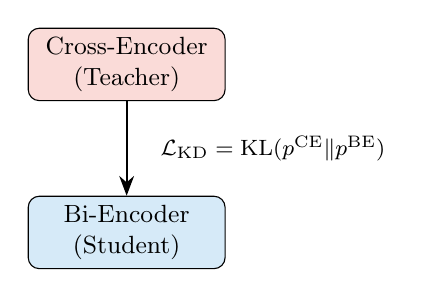
\begin{tikzpicture}[
    box/.style={draw, rounded corners, fill=#1, minimum height=0.8cm, minimum width=2.5cm, align=center, font=\small},
    arr/.style={-{Stealth[length=2.5mm]}, thick}
]
\node[box=dense!20] (ce) {Cross-Encoder\\(Teacher)};
\node[box=sparse!20, below=1.2cm of ce] (be) {Bi-Encoder\\(Student)};

\draw[arr] (ce) -- (be) node[midway, right, font=\footnotesize, xshift=0.3cm] {$\mathcal{L}_{\text{KD}} = \text{KL}(p^{\text{CE}} \| p^{\text{BE}})$};
\end{tikzpicture}
\end{center}

\vspace{0.5em}

\begin{block}{Process}
\begin{enumerate}
    \item Train cross-encoder on MS MARCO (high accuracy)
    \item Use cross-encoder to score top-$k$ BM25 passages for each query
    \item Train bi-encoder to \textbf{mimic} cross-encoder's ranking (soft labels)
\end{enumerate}
\end{block}

\textbf{Result:} Bi-encoder approaches cross-encoder quality at bi-encoder speed. This is how production systems like TAS-B are trained.
\end{frame}

\begin{frame}{Backup: Open Research Frontiers}
\begin{enumerate}
    \item \textbf{Closing the BEIR gap}
    \begin{itemize}
        \item Contriever, RetroMAE: unsupervised pre-training
        \item E5, GTE: instruction-tuned retrievers
    \end{itemize}

    \vspace{0.3em}

    \item \textbf{Scaling to billions of documents}
    \begin{itemize}
        \item Binary quantization, product quantization
        \item Matryoshka representations (flexible dimensionality)
    \end{itemize}

    \vspace{0.3em}

    \item \textbf{Multimodal retrieval}
    \begin{itemize}
        \item CLIP for image--text retrieval
        \item ColPali: late interaction for document images
    \end{itemize}

    \vspace{0.3em}

    \item \textbf{Integration with LLMs}
    \begin{itemize}
        \item Retrieval-augmented generation (RAG)
        \item LLM-based re-ranking (RankGPT from Lecture 4 backup)
    \end{itemize}
\end{enumerate}
\end{frame}

\begin{frame}{References}
\footnotesize
\begin{itemize}
    \item Karpukhin et al.\ (2020). Dense Passage Retrieval for Open-Domain QA. \textit{EMNLP}.
    \item Khattab \& Zaharia (2020). ColBERT: Efficient and Effective Passage Search. \textit{SIGIR}.
    \item Xiong et al.\ (2021). Approximate Nearest Neighbor Negative Contrastive Learning for Dense Text Retrieval. \textit{ICLR}.
    \item Reimers \& Gurevych (2019). Sentence-BERT. \textit{EMNLP}.
    \item Oord et al.\ (2018). Representation Learning with Contrastive Predictive Coding. \textit{arXiv}.
    \item Izacard et al.\ (2022). Unsupervised Dense Information Retrieval with Contrastive Learning. \textit{TMLR}.
    \item Thakur et al.\ (2021). BEIR: A Heterogeneous Benchmark for Zero-shot IR. \textit{NeurIPS Datasets}.
    \item Papyan et al.\ (2020). Prevalence of Neural Collapse. \textit{PNAS}.
    \item Tishby et al.\ (2000). The Information Bottleneck Method. \textit{Allerton}.
    \item Hofst\"atter et al.\ (2021). Efficiently Teaching an Effective Dense Retriever. \textit{SIGIR}.
\end{itemize}
\end{frame}

\end{document}
